
\documentclass[11pt,journal]{IEEEtran}


\usepackage{cite}
\usepackage[pdftex]{graphicx}
\usepackage[tight,footnotesize]{subfigure}
\usepackage{fixltx2e}
\usepackage{float}
\usepackage{url}

% correct bad hyphenation here
\hyphenation{op-tical net-works semi-conduc-tor}


\begin{document}

\title{CSE 471 Project Write-up \\ Team 2}

\author{\IEEEauthorblockN{David Ganey, Kerry Martin, Evan Stoll, Michael Theut, and Ben Roos\\}
\IEEEauthorblockA{School of Computing, Informatics and Decision Systems Engineering\\
Arizona State University\\
CSE 471\\}
}

% make the title area
\maketitle

\renewcommand{\abstractname}{Executive Summary}
\begin{abstract}
The CEO of CactusCard has commissioned a team to solve several problems facing the up-and-coming financial company. The company is in the process of releasing a new card, called the CactusCardPlus. In order for this new product to be a success, the CEO recognizes that CactusCard Credit must accomplish three distinct goals. First, the company needs to successfully market the new card, through both traditional strategies and in particular to users of social media. In addition to a powerful marketing campaign, the company must ensure it makes good decisions about which applicants are deserving of a line of credit. Failing to do this would put the company at a disadvantage, relative to the numerous credit agencies who do use data to make credit decisions. Finally, the success of the product hinges on its ability to protect users (and the company) from credit card fraud. As such, the team must be prepared to counter fraudulent users through a variety of strategies.
\par
These tasks will be undertaken by a team of computer science students with knowledge of artificial intelligence. Using search algorithms, the team will maximize the marketing potential of the card. Using machine learning techniques, the team will utilize data to accurately predict which applicants will best utilize their line of credit. Using game theory, the team will develop successful counter-fraud strategies which can be used to protect the company. 
\par
First, the team needed to market the card effectively. Using 10 cards with no sign up fee and 0\% interest for one year, CactusCard Credit strategically generated interest in the product. Using search techniques described below in Section \ref{part1}, the team devised both simple and complex algorithms which find the optimum individuals to receive these free cards in order to maximize the number of their friends who sign up for the product. The team found that TODO FILL THIS IN was the best algorithm for this, as it BLAH BLAH DETAILS.
\par
After devising a successful marketing strategy, the team turned its focus to the determination of credit worthiness. As seen below in Section \ref{part2}, the team used a well-known machine learning library called Weka to run various machine learning algorithms on the data set provided. This data set, which contained 15 anonymized credit attributes plus whether or not that individual was given a card, was used to train learning machines which were then evaluated on their ability to accurately predict the issuance decision. The team found that a machine running the Multilayer Perceptron algorithm was the most successful at predicting credit decisions and would serve the company well in the future.
\par
Paragraph(s) about the game theory part
\end{abstract}
\newpage

\IEEEpeerreviewmaketitle

\section{Part 1} \label{part1}
The first part of the project requires the development of search programs to optimize marketing within a social network. Using a dataset given to the study team by the marketing department, the team must propose multiple search-based solutions and document their success. This section will formulate this problem and describe the steps taken to solve it.

\subsection{Problem Importance}
For a new product such as the CactusCard Plus, the initial marketing wave may determine whether the product success or fails. This importance of this period, as the product begins to build a user base, cannot be overstated. Even more critical is the fact that the marketing department wishes to give out some of the cards for free. It is critical that the team choose the right users to receive these free cards such that the impact of those cards in their friend network is the largest.

\subsection{Solution Proposals}
The social network information given by the marketing department takes the form of a graph of friends. Each row of the dataset indicates a bidirectional relationship between two individuals. The goal is to give out one free card per day for 10 days. After giving a card, we can track the friends of the individual who received the card (``exposed" individuals) and determine the probability that they sign up for CactusCard Plus. Strategically distributing these cards in the friend network will maximize the number of sign ups, while never putting the company in a position where it has to give a free card to a friend of an individual who already received a free card (as that is unlikely to net new sign ups).
\par
Two solutions are proposed. The first solution to this search problem uses a simple depth-first search. TODO -- expand more on this here.

\subsection{Test Plan}
TODO

\subsection{Solution 1}
TODO

\subsection{Solution 2}
TODO

\section{Part 2} \label{part2}
Part 2 of the project describes another task given by the CEO of the CactusCard Credit Company, wherein a program should be developed to provide ``a \emph{machine learning based approach} to identify individuals who should/should not be given the CactusCardPlus.'' This section will formulate this problem and describe the steps taken to solve it.

\subsection{Problem Importance}
The decision whether or not to grant a line of credit (and, as a corollary, how large that line of credit should be) is one of the most important decisions made by a credit agency. In this age of big data, agencies which fail to accurately utilize existing data to make these decisions are likely to fall behind agencies who are doing so. In this problem, CactusCard Credit is fortunate to have a dataset which tracks many credit attributes for a large number of users.

\subsection{Problem Formulation}
The problem itself is a machine-learning problem, which at its core simply means a program designed to recognize patterns. Machine learning can encompass a wide variety of problems, which can be divided into ``regression'' problems and ``classification'' problems. In this case, the consumer research division has given the team a dataset which contains information about customers \emph{for whom the decision to award or not to award the CactusCard has already been made}. This is important information -- because customers can either be given the card or not (a binary \emph{classification}), this falls under the realm of \emph{classification} machine learning problems. Additionally, the fact that the classification program will be trained with data means this is a \emph{supervised} learning problem.
\par
As a supervised classification machine, the program must be able to read the data set and, with that information, draw conclusions about which credit variables have the largest impact on whether or not the customer was given the card. To be an effective tool for the CactusCard corporation, the dataset supplied by the consumer research division should only include proper decisions -- cases where the card was awarded to the correct individual and denied to individuals who would have abused the line of credit. Otherwise, the machine will learn ``bad habits'' and will draw conclusions from the data which are not useful to the company.
\par
The dataset itself is comprised of 15 credit attributes for the individuals, as well as an indication of whether the individual received a card. The credit attributes are not specified, though the problem specification does include the data types for each attribute. (For example, attribute 1 can be either ``b'' or ``a'', and therefore represents some binary information about the customer such as whether they are male or female). These attributes, therefore, are all weighted equally, which may present a disadvantage. Further discussion of this issue can be found in Section \ref{conclusion}. Additionally, it is important to note that the dataset is approximately balanced --- approximately half of the individuals were granted cards, while half were not. This is helpful in correctly training the classifier.
\par
The goal of this component of the project is to determine an algorithm which will effectively use the dataset to learn how the credit attributes affect the decision to award the card, and from there use that knowledge to predict card decisions within a certain degree of accuracy.

\subsection{Solution Proposals}
Weka, a software tool developed at the University of Waikato, is a software package with implementations of a large number of machine learning algorithms. Weka can be used in multiple ways. One option is to simply use the Weka API to access the algorithms from Java code. This is advantageous when one wishes to write a full machine learning system, or integrate machine learning algorithms with an existing Java system. Another option is to use the Weka Explorer, which is a wrapper around the algorithms. This GUI tool allows the user to load a data set and run the algorithms on it, then view the results in various formats.
\par
It is the latter method which is proposed to solve the task given by the CEO. Using the Weka Explorer, we have a straightforward method for gaining insight into the effect of the 15 credit attributes. We can use the Explorer to test various machine learning algorithms, and based on their success rates, determine which should be used in the future to make the actual issue decision. An additional advantage of using this method is that Weka is tested, proven, open-source code. The GitHub repository has nearly 8,000 commits, and therefore represents much more stable code than the team could have produced in the time allotted to this study \cite{wekagit}. This provides greater value for the company.

\begin{figure}[H]
\centering
    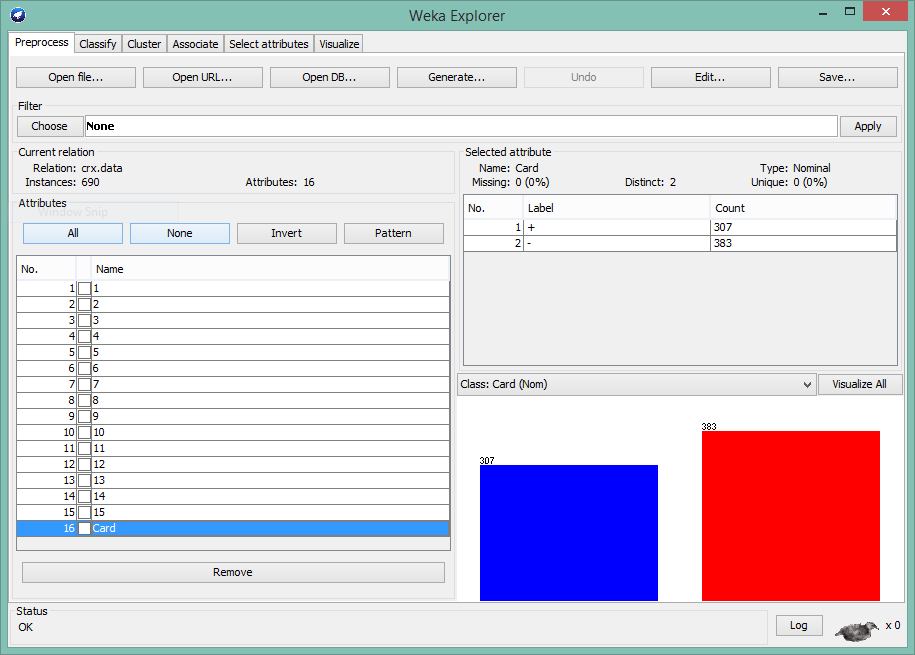
\includegraphics[width=3in]{images/wekaexplorer}
\caption{The Weka Explorer interface}
\label{wekaexplorer}
\end{figure}

\subsection{Test Plan} \label{testplan}
The team will evaluate several popular machine learning algorithms in the Weka Explorer. The success of each algorithm will be determined by a number of factors. The team must consider runtime, as the algorithm cannot take an extreme amount of time to complete or it will be useless. The most important factor, however, is the accuracy of the classification. Using random chance to classify card issuance would theoretically have an accuracy rate of approximately 50\%, so the team must find an algorithm with a higher percentage than that. To ensure CactusCard's continued financial success, the algorithm must predict card issuance correctly at least 80\% of the time. The team proposes this number as it represents a realistic target for algorithms which make mistakes, yet still shows a tremendous potential advantage for CactusCard Credit.

\subsection{Solution 1}
Support Vector Machines (SVM) are, according to Russell and Norvig, ``the most popular approach for `off-she-shelf' supervised learning''' \cite{ai}. SVMs do a good job of classification because they separate groups as much as possible (called a ``maximum margin separator''). Additionally, SVMs can work in multiple dimensions (creating a ``hyperplane'') which will be important with the high number of credit attributes in the data set. Finally, SVMs are considered a non-parametric method, because they store some of the training examples, and yet like parametric models, they often avoid over-fitting the data \cite{ai}.
\par
To use an SVM on the data set provided by the CEO, Weka supports the addition of a library called libsvm. This Java library contains an implementation of the SVM algorithm which hooks into the Weka Explorer interface. The team will set the Explorer to use varying numbers of crossfold validation passes, in order to evaluate the classifier. This will split the dataset, train the SVM with a subset of the dataset, and then evaluate the SVM's effectiveness at predicting the card issuance decision by comparing the SVM's predictions to the actual data. The results from running the libsvm algorithm on the dataset are shown in the table below:

\begin{table}[H]
{\renewcommand{\arraystretch}{1.2}%
\begin{tabular}{ | p{2.5cm} | l | l | l | }
\hline
Crossfold validations         & 5             & 10            & 15            \\ \hline
Time taken to build model (s) & .19           & .24           & .19           \\ \hline
Correctly classified (\%)     & 382 (55.36\%) & 385 (55.80\%) & 384 (55.65\%) \\ \hline
Incorrectly classified (\%)   & 308 (44.64\%) & 305 (44.20\%) & 306 (44.35\%) \\ \hline
\end{tabular}} \quad
\caption{A table showing the results of the libsvm applied to the data set}
\end{table}

As we can see from the table, no significant difference exists when adjusting the number of crossfold validation passes. All of the attempts fall well within the expected runtime, and predict with approximately 55\% accuracy whether someone was or was not given a CactusCard. While this is consistently better than randomly guessing, it only exceeds that percentage by approximately 5\%. While SVMs are good classifiers, in this instance this algorithm is not a suitable choice for the company, as it fails the 80\% criteria established in Section \ref{testplan}.

\subsection{Solution 2}
Another type of machine learning algorithm is called a Multilayer Perceptron (MLP). This is a type of neural network, which maps from inputs (in this case, the credit attributes) to outputs (whether someone was given a card). The MLP is suitable for this task because it uses \emph{backpropagation}, which is a supervised learning technique. The network is initialized with random initial weights, then backpropagation algorithm minimizes the error function using the method of gradient descent, which in turn recursively updates the initial weights. By using backpropagation, MLPs are able to handle hidden values which are present in this dataset. Given that MLPs handle such hidden values whereas SVMs do not, we intuitively expect that MLPs will better classify the data.
\par
The Multilayer Perceptron is significantly more complex than the SVM, but conveniently Weka does include an implementation in the Explorer. Using the same technique as above, the team will evaluate this algorithm with various levels of crossfold validation to determine the optimal setting. The results are seen below:

\begin{table}[H]
{\renewcommand{\arraystretch}{1.2}%
	\begin{tabular}{ | p{2.5cm} | l | l | l | }
\hline
Crossfold validations         & 5             & 10            & 15            \\ \hline
Time taken to build model (s) & 8.46          & 8.47          & 8.51          \\ \hline
Correctly classified (\%)     & 584 (84.64\%) & 572 (82.90\%) & 572 (82.90\%) \\ \hline
Incorrectly classified (\%)   & 106 (15.36\%) & 118 (17.10\%) &           118 (17.10\%)  \\ \hline
\end{tabular}
} \quad
\caption{A table showing the results of the Multilayer Perceptron applied to the data set}
\label{fig:mlp}
\end{table}

Once again, it is clear that adjusting the number of crossfold validations has little to no effect on the accuracy of the classifier. As a result, the recommendation of the team is to use 5 validations on data sets of this size, so the algorithm does not take too long to run. While the time taken to build the data model was always nearly the same, the total runtime for all passes of the validation increased dramatically with larger numbers of cross fold validations. Since they appear to have no impact on the effectiveness of the algorithm, there is no need for the program to take that additional time. It is likely that on future datasets with larger numbers of individuals, the runtime would increase further still, reinforcing the decision that 5 crossfold validations is the correct choice.
\par
Although no difference between the columns in Table \ref{fig:mlp} is visible, we can see immediately that the Multilayer Perceptron is a good choice for the CactusCard company. In all cases, the success of the classifier was above the criteria set above in Section \ref{testplan}. The MLP algorithm averaged approximately 83\% correctness, which is significantly higher than random chance. This algorithm would be a good choice for future data sets, where it could use the information it learned from this training set to choose who receives a card.

\section{Part 3} \label{part3}
\subsection{Dominant Strategy}

Whenever this game is played, CactusCard cannot make money. Since CactusCard can only lose money, the goal then is to make sure that the game is played for the shortest amount of time possible. The most cost-effective way to make sure the game is not played very long is to make sure the attacker is not making any money, and then minimizing our cost while still ensuring that the attacker is not making money.
\par
So the goal is to defend the number of attacks that will maximize his losses and minimize the money we spend. 
\par
The first priority is to ensure the attacker is losing money. This is computed through determining the expected value. Once we get him losing money, we need to find the optimal amount of vectors to defend that will minimize out losses. The following is our findings when the attacker attacks 1, 2, and 10 vectors.
\par
Assuming:
attacker = 1,
catk = 1000
\par
cost results: 

Defender $\Rightarrow$ Assuming they only attack one vector, then we're going to average out to about -\$10000 anyway we play, no matter what the other variables are. The best results I found were defending 97 attacks. That way, the attacker will average out at -\$797.98 and the defender will average out at -\$9902.02.
\par
Assuming:
attacker = 2,
catk = 500
\par
cost results: 

Defender $\Rightarrow$ The attacker's next best move is to attack 2 vectors. This time, the most cost effective way to ensure that he doesn't average out to make any money is to defend 68 vectors. This averages out to the defender losing \$41.43 and the attacker losing \$41.43 and the defender losing \$7758.77
\par
Assuming:
attacker = 10,
catk = 300
\par
cost results: 

Defender $\Rightarrow$ This time the attacker attacks 10 vectors. The best response when the defender is paying \$300 per attack is to defend 22 vectors. This still gives a likelihood of defense at 92.96\% and averages out the defender to lose \$2192.31 per round the defender to lose \$2907.69
\par
Overall, the reasonable investment for the company entirely depends on the amount of attack vectors that the attacker decides to play. The fewer he plays, the more expensive it is for the company.



\section{Conclusion} \label{conclusion}
The conclusion goes here.
Discuss issues with part 2 dataset -- all attributes weighted equally



% conference papers do not normally have an appendix


% use section* for acknowledgement
\section*{Appendices}

Source code and stuff goes here


\begin{thebibliography}{1}

\bibitem{IEEEhowto:kopka}
H.~Kopka and P.~W. Daly, \emph{A Guide to \LaTeX}, 3rd~ed.\hskip 1em plus
  0.5em minus 0.4em\relax Harlow, England: Addison-Wesley, 1999.

\end{thebibliography}



% that's all folks
\end{document}


